Table with
high level objectives

Specific objective

Activity of achiete this objective

KPI (Results and way to measure it)





{\color{red} include KPI} LIL are KPI's





To foster the interoperability of proof systems and the sustainability
and the cross-verification of formal proofs, we propose to collect
them in an online encyclopedia, called Logipedia.  For each proof,
Logipedia will indicate in which systems it can be used and, when this
is the case, it will provide a version of this proof in the theory of
these systems.

Such a project will not only foster the use of formal proofs in
research in mathematics and computer science, but also in industry, by
allowing cross-verification, sustainability, and interoperability of
formal proofs, and in education, freeing the teaching of formal proof
technology from being bound to one system.

Such a project can only have a worldwide ambition. However, as a
majority of proof systems are developed in Europe, there is a unique
opportunity for Europe to take the lead on such a project and prepare
the grounds for the economic spinoffs from the project benefiting
European industry. That is why the consortium gathers most of the
European actors active on formal proof systems, while also developing
links with non-European partners.

The ultimate goal of Logipedia is to have all the formal proofs
available to mankind in a single encyclopedia.  A first proof of
concept contains a few hundred lemmas, from the Matita library,
expressed in the logic of six different systems: Matita, Coq, Lean,
HOL Light, Isabelle/HOL, and PVS.  In the next four years, we plan to
address, with different ambitions, the libraries of Agda, Atelier B,
Coq, FoCaLiZe, HOL Light, HOL4, Isabelle, Matita, Minlog, Mizar, ProB,
PVS, Rodin, TLA+, and Why3.  Beyond our main focus on interactive
systems, we also plan to integrate some proofs coming from automated
theorem provers, SMT solvers, and model checkers, when these proofs
have a manageable size.

Building this encyclopedia is {\em per se} a networking activity
between the partners, from academia and industry, involved in the
project.

Logipedia will be freely accessible through a web browser, from any
country in Europe and beyond. So, by construction, the access will be
trans-national and virtual. But beyond these two objectives of a
trans-national and virtual access, an important effort will be made to
make this encyclopedia accessible to a large community of specialists
and non-specialists. This requires to develop an ergonomic web
interface and a package distribution system, to develop a search
engine, and to structure the content of the encyclopedia into
libraries, books, chapters, etc., reaping the benefit of the structure
(modules, qualified names, etc.) of some of the libraries we start
with.

Finally, this project will trigger joint research activities between
its users and between its developers.  

First, if the theories implemented in some systems have already been
understood, so that the integration of the proofs expressed in these
systems and their translation to other theories, will be made
smoothly, for others, more research work is needed. 

A research effort will also be made to engineer these proofs: analyze
the axioms they use, translate them into other theories, etc.  In
addition, each library contains definitions of natural numbers, real
numbers, etc. that we will align: structural results proved for one
definition of real numbers, for instance, will be transported to any
isomorphic structure, regardless the way it has been defined.

All these objectives contribute to building a new formal proof
community, focused on the values of
knowledge sharing, safety, security, privacy, open access, education, etc.

\newpage

\begin{framed}
\begin{center}
{\bf Main objectives}
\end{center}

\begin{tabular}{l}
  Integration of proof systems\\
  Integration of automated theorem proving\\
  Integration of libraries\\
  \\
  Development of the infrastructure\\
  Structuring the infrastuture\\
  \\
  New theories, new systems\\
  Proof engineering\\
\end{tabular}
\end{framed}


\begin{framed}

\begin{center}
{\bf \Large History of the project}
\end{center}

Convinced that a cloud of formal proofs could bring to the
applications of formal proof technology the same boost that the cloud
has brought to computing, and also that managing a large encyclopedia
required some interdisciplinary effort, 
we developed a proof of concept containing a few hundreds lemmas 
expressed in the language of six systems and organized, in January 2019,
a meeting to discuss the future of this project.
This
meeting brought together 38 researchers from Austria, the Czech
Republic, France, Italy, the Netherlands, and Poland, some of them 
being from the TYPES community, others not.
\begin{center}
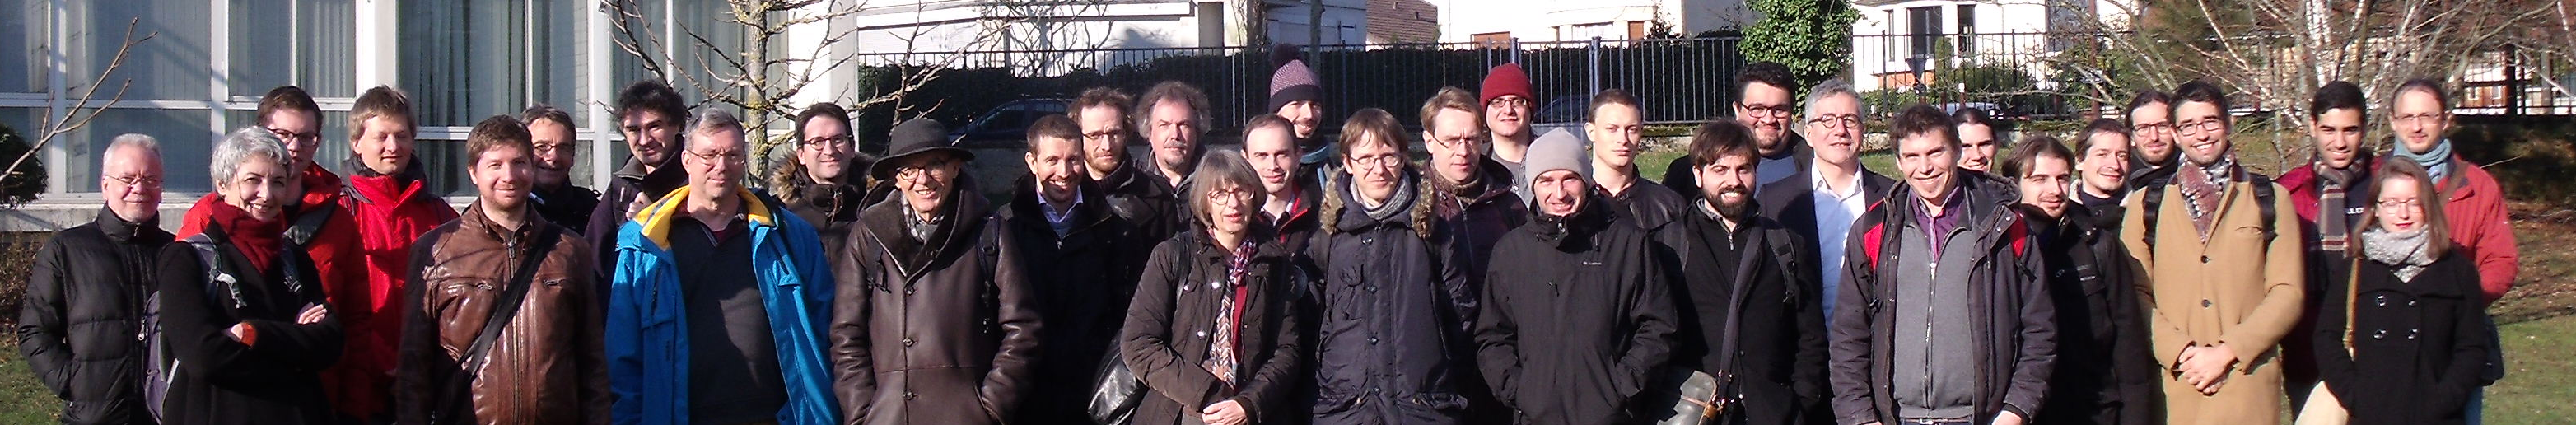
\includegraphics[height=2cm]{photo.png}
\end{center}
During this meeting, the idea of making this proof of concept a European 
infrastructure emerged.
Since then,
colleagues from Belgium, Germany, Serbia, Sweden, and the United
Kingdom, from academia and industry, have manifested interest in
participating in this effort.  These researchers and engineers are
ready to contribute to develop this encyclopedia, aiming at sharing
proofs, under a creative common licence making them findable,
accessible, interoperable, and reusable.

\end{framed}

%%% Local Variables:
%%%   mode: latex
%%%   mode: flyspell
%%%   ispell-local-dictionary: "english"
%%% End:

